\documentclass[twoside]{book}

% Packages required by doxygen
\usepackage{fixltx2e}
\usepackage{calc}
\usepackage{doxygen}
\usepackage[export]{adjustbox} % also loads graphicx
\usepackage{graphicx}
\usepackage[utf8]{inputenc}
\usepackage{makeidx}
\usepackage{multicol}
\usepackage{multirow}
\PassOptionsToPackage{warn}{textcomp}
\usepackage{textcomp}
\usepackage[nointegrals]{wasysym}
\usepackage[table]{xcolor}

% Font selection
\usepackage[T1]{fontenc}
\usepackage[scaled=.90]{helvet}
\usepackage{courier}
\usepackage{amssymb}
\usepackage{sectsty}
\renewcommand{\familydefault}{\sfdefault}
\allsectionsfont{%
  \fontseries{bc}\selectfont%
  \color{darkgray}%
}
\renewcommand{\DoxyLabelFont}{%
  \fontseries{bc}\selectfont%
  \color{darkgray}%
}
\newcommand{\+}{\discretionary{\mbox{\scriptsize$\hookleftarrow$}}{}{}}

% Page & text layout
\usepackage{geometry}
\geometry{%
  a4paper,%
  top=2.5cm,%
  bottom=2.5cm,%
  left=2.5cm,%
  right=2.5cm%
}
\tolerance=750
\hfuzz=15pt
\hbadness=750
\setlength{\emergencystretch}{15pt}
\setlength{\parindent}{0cm}
\setlength{\parskip}{3ex plus 2ex minus 2ex}
\makeatletter
\renewcommand{\paragraph}{%
  \@startsection{paragraph}{4}{0ex}{-1.0ex}{1.0ex}{%
    \normalfont\normalsize\bfseries\SS@parafont%
  }%
}
\renewcommand{\subparagraph}{%
  \@startsection{subparagraph}{5}{0ex}{-1.0ex}{1.0ex}{%
    \normalfont\normalsize\bfseries\SS@subparafont%
  }%
}
\makeatother

% Headers & footers
\usepackage{fancyhdr}
\pagestyle{fancyplain}
\fancyhead[LE]{\fancyplain{}{\bfseries\thepage}}
\fancyhead[CE]{\fancyplain{}{}}
\fancyhead[RE]{\fancyplain{}{\bfseries\leftmark}}
\fancyhead[LO]{\fancyplain{}{\bfseries\rightmark}}
\fancyhead[CO]{\fancyplain{}{}}
\fancyhead[RO]{\fancyplain{}{\bfseries\thepage}}
\fancyfoot[LE]{\fancyplain{}{}}
\fancyfoot[CE]{\fancyplain{}{}}
\fancyfoot[RE]{\fancyplain{}{\bfseries\scriptsize Generated by Doxygen }}
\fancyfoot[LO]{\fancyplain{}{\bfseries\scriptsize Generated by Doxygen }}
\fancyfoot[CO]{\fancyplain{}{}}
\fancyfoot[RO]{\fancyplain{}{}}
\renewcommand{\footrulewidth}{0.4pt}
\renewcommand{\chaptermark}[1]{%
  \markboth{#1}{}%
}
\renewcommand{\sectionmark}[1]{%
  \markright{\thesection\ #1}%
}

% Indices & bibliography
\usepackage{natbib}
\usepackage[titles]{tocloft}
\setcounter{tocdepth}{3}
\setcounter{secnumdepth}{5}
\makeindex

% Hyperlinks (required, but should be loaded last)
\usepackage{ifpdf}
\ifpdf
  \usepackage[pdftex,pagebackref=true]{hyperref}
\else
  \usepackage[ps2pdf,pagebackref=true]{hyperref}
\fi
\hypersetup{%
  colorlinks=true,%
  linkcolor=blue,%
  citecolor=blue,%
  unicode%
}

% Custom commands
\newcommand{\clearemptydoublepage}{%
  \newpage{\pagestyle{empty}\cleardoublepage}%
}

\usepackage{caption}
\captionsetup{labelsep=space,justification=centering,font={bf},singlelinecheck=off,skip=4pt,position=top}

%===== C O N T E N T S =====

\begin{document}

% Titlepage & ToC
\hypersetup{pageanchor=false,
             bookmarksnumbered=true,
             pdfencoding=unicode
            }
\pagenumbering{alph}
\begin{titlepage}
\vspace*{7cm}
\begin{center}%
{\Large Scientific\+\_\+\+Calculator }\\
\vspace*{1cm}
{\large Generated by Doxygen 1.8.13}\\
\end{center}
\end{titlepage}
\clearemptydoublepage
\pagenumbering{roman}
\tableofcontents
\clearemptydoublepage
\pagenumbering{arabic}
\hypersetup{pageanchor=true}

%--- Begin generated contents ---
\chapter{Namespace Index}
\section{Packages}
Here are the packages with brief descriptions (if available)\+:\begin{DoxyCompactList}
\item\contentsline{section}{\hyperlink{namespace_scientific___calculator}{Scientific\+\_\+\+Calculator} }{\pageref{namespace_scientific___calculator}}{}
\item\contentsline{section}{\hyperlink{namespace_scientific___calculator_1_1_properties}{Scientific\+\_\+\+Calculator.\+Properties} }{\pageref{namespace_scientific___calculator_1_1_properties}}{}
\end{DoxyCompactList}

\chapter{Hierarchical Index}
\section{Class Hierarchy}
This inheritance list is sorted roughly, but not completely, alphabetically\+:\begin{DoxyCompactList}
\item \contentsline{section}{Scientific\+\_\+\+Calculator.\+Calculation}{\pageref{class_scientific___calculator_1_1_calculation}}{}
\item \contentsline{section}{Scientific\+\_\+\+Calculator.\+D\+B\+Access}{\pageref{class_scientific___calculator_1_1_d_b_access}}{}
\item Form\begin{DoxyCompactList}
\item \contentsline{section}{Scientific\+\_\+\+Calculator.\+frm\+Calculator}{\pageref{class_scientific___calculator_1_1frm_calculator}}{}
\item \contentsline{section}{Scientific\+\_\+\+Calculator.\+frm\+Function\+Plot}{\pageref{class_scientific___calculator_1_1frm_function_plot}}{}
\item \contentsline{section}{Scientific\+\_\+\+Calculator.\+frm\+History}{\pageref{class_scientific___calculator_1_1frm_history}}{}
\item \contentsline{section}{Scientific\+\_\+\+Calculator.\+frm\+Settings}{\pageref{class_scientific___calculator_1_1frm_settings}}{}
\end{DoxyCompactList}
\end{DoxyCompactList}

\chapter{Class Index}
\section{Class List}
Here are the classes, structs, unions and interfaces with brief descriptions\+:\begin{DoxyCompactList}
\item\contentsline{section}{\hyperlink{class_scientific___calculator_1_1_calculation}{Scientific\+\_\+\+Calculator.\+Calculation} \\*Class that handles all the mathematics of the program, and interpretes the operations inputs }{\pageref{class_scientific___calculator_1_1_calculation}}{}
\item\contentsline{section}{\hyperlink{class_scientific___calculator_1_1_d_b_access}{Scientific\+\_\+\+Calculator.\+D\+B\+Access} \\*Class that handles all the database operations }{\pageref{class_scientific___calculator_1_1_d_b_access}}{}
\item\contentsline{section}{\hyperlink{class_scientific___calculator_1_1frm_calculator}{Scientific\+\_\+\+Calculator.\+frm\+Calculator} \\*Main form, contains the calculator itself and buttons to open all the other forms as dialog windows }{\pageref{class_scientific___calculator_1_1frm_calculator}}{}
\item\contentsline{section}{\hyperlink{class_scientific___calculator_1_1frm_function_plot}{Scientific\+\_\+\+Calculator.\+frm\+Function\+Plot} \\*Form that displays a graph from a given function }{\pageref{class_scientific___calculator_1_1frm_function_plot}}{}
\item\contentsline{section}{\hyperlink{class_scientific___calculator_1_1frm_history}{Scientific\+\_\+\+Calculator.\+frm\+History} \\*Form that displays the operations history on a listbox }{\pageref{class_scientific___calculator_1_1frm_history}}{}
\item\contentsline{section}{\hyperlink{class_scientific___calculator_1_1frm_settings}{Scientific\+\_\+\+Calculator.\+frm\+Settings} \\*Form that allows the user to change some application settings }{\pageref{class_scientific___calculator_1_1frm_settings}}{}
\end{DoxyCompactList}

\chapter{File Index}
\section{File List}
Here is a list of all files with brief descriptions\+:\begin{DoxyCompactList}
\item\contentsline{section}{C\+:/\+Scientific\+\_\+\+Calculator/\+Scientific\+\_\+\+Calculator/\+Code/\+Scientific\+\_\+\+Calculator/\+Scientific\+\_\+\+Calculator/\hyperlink{_calculation_8cs}{Calculation.\+cs} }{\pageref{_calculation_8cs}}{}
\item\contentsline{section}{C\+:/\+Scientific\+\_\+\+Calculator/\+Scientific\+\_\+\+Calculator/\+Code/\+Scientific\+\_\+\+Calculator/\+Scientific\+\_\+\+Calculator/\hyperlink{_d_b_access_8cs}{D\+B\+Access.\+cs} }{\pageref{_d_b_access_8cs}}{}
\item\contentsline{section}{C\+:/\+Scientific\+\_\+\+Calculator/\+Scientific\+\_\+\+Calculator/\+Code/\+Scientific\+\_\+\+Calculator/\+Scientific\+\_\+\+Calculator/\hyperlink{frm_calculator_8cs}{frm\+Calculator.\+cs} }{\pageref{frm_calculator_8cs}}{}
\item\contentsline{section}{C\+:/\+Scientific\+\_\+\+Calculator/\+Scientific\+\_\+\+Calculator/\+Code/\+Scientific\+\_\+\+Calculator/\+Scientific\+\_\+\+Calculator/\hyperlink{frm_calculator_8_designer_8cs}{frm\+Calculator.\+Designer.\+cs} }{\pageref{frm_calculator_8_designer_8cs}}{}
\item\contentsline{section}{C\+:/\+Scientific\+\_\+\+Calculator/\+Scientific\+\_\+\+Calculator/\+Code/\+Scientific\+\_\+\+Calculator/\+Scientific\+\_\+\+Calculator/\hyperlink{frm_function_plot_8cs}{frm\+Function\+Plot.\+cs} }{\pageref{frm_function_plot_8cs}}{}
\item\contentsline{section}{C\+:/\+Scientific\+\_\+\+Calculator/\+Scientific\+\_\+\+Calculator/\+Code/\+Scientific\+\_\+\+Calculator/\+Scientific\+\_\+\+Calculator/\hyperlink{frm_function_plot_8_designer_8cs}{frm\+Function\+Plot.\+Designer.\+cs} }{\pageref{frm_function_plot_8_designer_8cs}}{}
\item\contentsline{section}{C\+:/\+Scientific\+\_\+\+Calculator/\+Scientific\+\_\+\+Calculator/\+Code/\+Scientific\+\_\+\+Calculator/\+Scientific\+\_\+\+Calculator/\hyperlink{frm_history_8cs}{frm\+History.\+cs} }{\pageref{frm_history_8cs}}{}
\item\contentsline{section}{C\+:/\+Scientific\+\_\+\+Calculator/\+Scientific\+\_\+\+Calculator/\+Code/\+Scientific\+\_\+\+Calculator/\+Scientific\+\_\+\+Calculator/\hyperlink{frm_history_8_designer_8cs}{frm\+History.\+Designer.\+cs} }{\pageref{frm_history_8_designer_8cs}}{}
\item\contentsline{section}{C\+:/\+Scientific\+\_\+\+Calculator/\+Scientific\+\_\+\+Calculator/\+Code/\+Scientific\+\_\+\+Calculator/\+Scientific\+\_\+\+Calculator/\hyperlink{frm_settings_8cs}{frm\+Settings.\+cs} }{\pageref{frm_settings_8cs}}{}
\item\contentsline{section}{C\+:/\+Scientific\+\_\+\+Calculator/\+Scientific\+\_\+\+Calculator/\+Code/\+Scientific\+\_\+\+Calculator/\+Scientific\+\_\+\+Calculator/\hyperlink{frm_settings_8_designer_8cs}{frm\+Settings.\+Designer.\+cs} }{\pageref{frm_settings_8_designer_8cs}}{}
\item\contentsline{section}{C\+:/\+Scientific\+\_\+\+Calculator/\+Scientific\+\_\+\+Calculator/\+Code/\+Scientific\+\_\+\+Calculator/\+Scientific\+\_\+\+Calculator/\hyperlink{_program_8cs}{Program.\+cs} }{\pageref{_program_8cs}}{}
\item\contentsline{section}{C\+:/\+Scientific\+\_\+\+Calculator/\+Scientific\+\_\+\+Calculator/\+Code/\+Scientific\+\_\+\+Calculator/\+Scientific\+\_\+\+Calculator/obj/\+Debug/\hyperlink{_temporary_generated_file__036_c0_b5_b-1481-4323-8_d20-8_f5_a_d_c_b23_d92_8cs}{Temporary\+Generated\+File\+\_\+036\+C0\+B5\+B-\/1481-\/4323-\/8\+D20-\/8\+F5\+A\+D\+C\+B23\+D92.\+cs} }{\pageref{_temporary_generated_file__036_c0_b5_b-1481-4323-8_d20-8_f5_a_d_c_b23_d92_8cs}}{}
\item\contentsline{section}{C\+:/\+Scientific\+\_\+\+Calculator/\+Scientific\+\_\+\+Calculator/\+Code/\+Scientific\+\_\+\+Calculator/\+Scientific\+\_\+\+Calculator/obj/\+Debug/\hyperlink{_temporary_generated_file__5937a670-0e60-4077-877b-f7221da3dda1_8cs}{Temporary\+Generated\+File\+\_\+5937a670-\/0e60-\/4077-\/877b-\/f7221da3dda1.\+cs} }{\pageref{_temporary_generated_file__5937a670-0e60-4077-877b-f7221da3dda1_8cs}}{}
\item\contentsline{section}{C\+:/\+Scientific\+\_\+\+Calculator/\+Scientific\+\_\+\+Calculator/\+Code/\+Scientific\+\_\+\+Calculator/\+Scientific\+\_\+\+Calculator/obj/\+Debug/\hyperlink{_temporary_generated_file___e7_a71_f73-0_f8_d-4_b9_b-_b56_e-8_e70_b10_b_c5_d3_8cs}{Temporary\+Generated\+File\+\_\+\+E7\+A71\+F73-\/0\+F8\+D-\/4\+B9\+B-\/\+B56\+E-\/8\+E70\+B10\+B\+C5\+D3.\+cs} }{\pageref{_temporary_generated_file___e7_a71_f73-0_f8_d-4_b9_b-_b56_e-8_e70_b10_b_c5_d3_8cs}}{}
\item\contentsline{section}{C\+:/\+Scientific\+\_\+\+Calculator/\+Scientific\+\_\+\+Calculator/\+Code/\+Scientific\+\_\+\+Calculator/\+Scientific\+\_\+\+Calculator/\+Properties/\hyperlink{_assembly_info_8cs}{Assembly\+Info.\+cs} }{\pageref{_assembly_info_8cs}}{}
\item\contentsline{section}{C\+:/\+Scientific\+\_\+\+Calculator/\+Scientific\+\_\+\+Calculator/\+Code/\+Scientific\+\_\+\+Calculator/\+Scientific\+\_\+\+Calculator/\+Properties/\hyperlink{_resources_8_designer_8cs}{Resources.\+Designer.\+cs} }{\pageref{_resources_8_designer_8cs}}{}
\item\contentsline{section}{C\+:/\+Scientific\+\_\+\+Calculator/\+Scientific\+\_\+\+Calculator/\+Code/\+Scientific\+\_\+\+Calculator/\+Scientific\+\_\+\+Calculator/\+Properties/\hyperlink{_settings_8_designer_8cs}{Settings.\+Designer.\+cs} }{\pageref{_settings_8_designer_8cs}}{}
\end{DoxyCompactList}

\chapter{Namespace Documentation}
\hypertarget{namespace_scientific___calculator}{}\section{Scientific\+\_\+\+Calculator Namespace Reference}
\label{namespace_scientific___calculator}\index{Scientific\+\_\+\+Calculator@{Scientific\+\_\+\+Calculator}}
\subsection*{Namespaces}
\begin{DoxyCompactItemize}
\item 
namespace \hyperlink{namespace_scientific___calculator_1_1_properties}{Properties}
\end{DoxyCompactItemize}
\subsection*{Classes}
\begin{DoxyCompactItemize}
\item 
class \hyperlink{class_scientific___calculator_1_1_calculation}{Calculation}
\begin{DoxyCompactList}\small\item\em Class that handles all the mathematics of the program, and interpretes the operations inputs \end{DoxyCompactList}\item 
class \hyperlink{class_scientific___calculator_1_1_d_b_access}{D\+B\+Access}
\begin{DoxyCompactList}\small\item\em Class that handles all the database operations \end{DoxyCompactList}\item 
class \hyperlink{class_scientific___calculator_1_1frm_calculator}{frm\+Calculator}
\begin{DoxyCompactList}\small\item\em Main form, contains the calculator itself and buttons to open all the other forms as dialog windows \end{DoxyCompactList}\item 
class \hyperlink{class_scientific___calculator_1_1frm_function_plot}{frm\+Function\+Plot}
\begin{DoxyCompactList}\small\item\em Form that displays a graph from a given function \end{DoxyCompactList}\item 
class \hyperlink{class_scientific___calculator_1_1frm_history}{frm\+History}
\begin{DoxyCompactList}\small\item\em Form that displays the operations history on a listbox \end{DoxyCompactList}\item 
class \hyperlink{class_scientific___calculator_1_1frm_settings}{frm\+Settings}
\begin{DoxyCompactList}\small\item\em Form that allows the user to change some application settings \end{DoxyCompactList}\item 
class {\bfseries Program}
\end{DoxyCompactItemize}

\hypertarget{namespace_scientific___calculator_1_1_properties}{}\section{Scientific\+\_\+\+Calculator.\+Properties Namespace Reference}
\label{namespace_scientific___calculator_1_1_properties}\index{Scientific\+\_\+\+Calculator.\+Properties@{Scientific\+\_\+\+Calculator.\+Properties}}
\subsection*{Classes}
\begin{DoxyCompactItemize}
\item 
class {\bfseries Resources}
\begin{DoxyCompactList}\small\item\em A strongly-\/typed resource class, for looking up localized strings, etc. \end{DoxyCompactList}\item 
class {\bfseries Settings}
\end{DoxyCompactItemize}

\chapter{Class Documentation}
\hypertarget{class_scientific___calculator_1_1_calculation}{}\section{Scientific\+\_\+\+Calculator.\+Calculation Class Reference}
\label{class_scientific___calculator_1_1_calculation}\index{Scientific\+\_\+\+Calculator.\+Calculation@{Scientific\+\_\+\+Calculator.\+Calculation}}


Class that handles all the mathematics of the program, and interpretes the operations inputs  


\subsection*{Public Member Functions}
\begin{DoxyCompactItemize}
\item 
double \hyperlink{class_scientific___calculator_1_1_calculation_ab4879c2e7890c6dfd7e954e6c424764f}{Solve} (string operation\+String)
\begin{DoxyCompactList}\small\item\em Sends the operation string to the Read\+Operation method, then sends the resulted array to the Calculate method, thus obtaining the numeric result. \end{DoxyCompactList}\end{DoxyCompactItemize}


\subsection{Detailed Description}
Class that handles all the mathematics of the program, and interpretes the operations inputs 



\subsection{Member Function Documentation}
\mbox{\Hypertarget{class_scientific___calculator_1_1_calculation_ab4879c2e7890c6dfd7e954e6c424764f}\label{class_scientific___calculator_1_1_calculation_ab4879c2e7890c6dfd7e954e6c424764f}} 
\index{Scientific\+\_\+\+Calculator\+::\+Calculation@{Scientific\+\_\+\+Calculator\+::\+Calculation}!Solve@{Solve}}
\index{Solve@{Solve}!Scientific\+\_\+\+Calculator\+::\+Calculation@{Scientific\+\_\+\+Calculator\+::\+Calculation}}
\subsubsection{\texorpdfstring{Solve()}{Solve()}}
{\footnotesize\ttfamily double Scientific\+\_\+\+Calculator.\+Calculation.\+Solve (\begin{DoxyParamCaption}\item[{string}]{operation\+String }\end{DoxyParamCaption})}



Sends the operation string to the Read\+Operation method, then sends the resulted array to the Calculate method, thus obtaining the numeric result. 


\begin{DoxyParams}{Parameters}
{\em operation\+String} & \\
\hline
\end{DoxyParams}
\begin{DoxyReturn}{Returns}

\end{DoxyReturn}


The documentation for this class was generated from the following file\+:\begin{DoxyCompactItemize}
\item 
C\+:/\+Scientific\+\_\+\+Calculator/\+Scientific\+\_\+\+Calculator/\+Code/\+Scientific\+\_\+\+Calculator/\+Scientific\+\_\+\+Calculator/\hyperlink{_calculation_8cs}{Calculation.\+cs}\end{DoxyCompactItemize}

\hypertarget{class_scientific___calculator_1_1_d_b_access}{}\section{Scientific\+\_\+\+Calculator.\+D\+B\+Access Class Reference}
\label{class_scientific___calculator_1_1_d_b_access}\index{Scientific\+\_\+\+Calculator.\+D\+B\+Access@{Scientific\+\_\+\+Calculator.\+D\+B\+Access}}


Class that handles all the database operations  


\subsection*{Public Member Functions}
\begin{DoxyCompactItemize}
\item 
\hyperlink{class_scientific___calculator_1_1_d_b_access_a6007d654070f5893e1876c19e1740a5c}{D\+B\+Access} ()
\begin{DoxyCompactList}\small\item\em Constructor that creates the connection to the database \end{DoxyCompactList}\item 
double \hyperlink{class_scientific___calculator_1_1_d_b_access_a55b2251a50067b4008e03b911770cdf7}{Get\+Constant} (string constant\+Name)
\begin{DoxyCompactList}\small\item\em Gets a chosen constant from the database \end{DoxyCompactList}\item 
int \hyperlink{class_scientific___calculator_1_1_d_b_access_a2b2a68c2a113ee7f4dabde92b4675d7e}{Get\+Default\+Setting} (string setting\+Name)
\begin{DoxyCompactList}\small\item\em Gets the default value of a chosen setting from the database \end{DoxyCompactList}\item 
void \hyperlink{class_scientific___calculator_1_1_d_b_access_a3ada18c0a3a5a48dd7b88b166b715c7d}{Update\+Setting} (string setting\+Name, int new\+Value)
\begin{DoxyCompactList}\small\item\em Updates the value of a chosen setting in the database \end{DoxyCompactList}\item 
int \hyperlink{class_scientific___calculator_1_1_d_b_access_a738341bafa087495fe4c940ef3c74517}{Get\+Setting\+Value} (string setting\+Name)
\begin{DoxyCompactList}\small\item\em Gets the current value of a chosen setting from the database \end{DoxyCompactList}\item 
List$<$ string $>$ \hyperlink{class_scientific___calculator_1_1_d_b_access_a0082501ed3f21914f17be60e4a7541b3}{Get\+Operation\+History} (int amount)
\begin{DoxyCompactList}\small\item\em Gets the latest operations from the operation history \end{DoxyCompactList}\item 
void \hyperlink{class_scientific___calculator_1_1_d_b_access_a9bfbf5393338345c6d5b41cb43fbc56b}{Insert\+Operation\+In\+History} (string Operation\+String)
\begin{DoxyCompactList}\small\item\em Inserts a new operation in the operation history dated to today \end{DoxyCompactList}\end{DoxyCompactItemize}


\subsection{Detailed Description}
Class that handles all the database operations 



\subsection{Constructor \& Destructor Documentation}
\mbox{\Hypertarget{class_scientific___calculator_1_1_d_b_access_a6007d654070f5893e1876c19e1740a5c}\label{class_scientific___calculator_1_1_d_b_access_a6007d654070f5893e1876c19e1740a5c}} 
\index{Scientific\+\_\+\+Calculator\+::\+D\+B\+Access@{Scientific\+\_\+\+Calculator\+::\+D\+B\+Access}!D\+B\+Access@{D\+B\+Access}}
\index{D\+B\+Access@{D\+B\+Access}!Scientific\+\_\+\+Calculator\+::\+D\+B\+Access@{Scientific\+\_\+\+Calculator\+::\+D\+B\+Access}}
\subsubsection{\texorpdfstring{D\+B\+Access()}{DBAccess()}}
{\footnotesize\ttfamily Scientific\+\_\+\+Calculator.\+D\+B\+Access.\+D\+B\+Access (\begin{DoxyParamCaption}{ }\end{DoxyParamCaption})}



Constructor that creates the connection to the database 



\subsection{Member Function Documentation}
\mbox{\Hypertarget{class_scientific___calculator_1_1_d_b_access_a55b2251a50067b4008e03b911770cdf7}\label{class_scientific___calculator_1_1_d_b_access_a55b2251a50067b4008e03b911770cdf7}} 
\index{Scientific\+\_\+\+Calculator\+::\+D\+B\+Access@{Scientific\+\_\+\+Calculator\+::\+D\+B\+Access}!Get\+Constant@{Get\+Constant}}
\index{Get\+Constant@{Get\+Constant}!Scientific\+\_\+\+Calculator\+::\+D\+B\+Access@{Scientific\+\_\+\+Calculator\+::\+D\+B\+Access}}
\subsubsection{\texorpdfstring{Get\+Constant()}{GetConstant()}}
{\footnotesize\ttfamily double Scientific\+\_\+\+Calculator.\+D\+B\+Access.\+Get\+Constant (\begin{DoxyParamCaption}\item[{string}]{constant\+Name }\end{DoxyParamCaption})}



Gets a chosen constant from the database 


\begin{DoxyParams}{Parameters}
{\em name} & the name of the constant we want to retrieve\\
\hline
\end{DoxyParams}
\begin{DoxyReturn}{Returns}
the numeric value of the constant
\end{DoxyReturn}
\mbox{\Hypertarget{class_scientific___calculator_1_1_d_b_access_a2b2a68c2a113ee7f4dabde92b4675d7e}\label{class_scientific___calculator_1_1_d_b_access_a2b2a68c2a113ee7f4dabde92b4675d7e}} 
\index{Scientific\+\_\+\+Calculator\+::\+D\+B\+Access@{Scientific\+\_\+\+Calculator\+::\+D\+B\+Access}!Get\+Default\+Setting@{Get\+Default\+Setting}}
\index{Get\+Default\+Setting@{Get\+Default\+Setting}!Scientific\+\_\+\+Calculator\+::\+D\+B\+Access@{Scientific\+\_\+\+Calculator\+::\+D\+B\+Access}}
\subsubsection{\texorpdfstring{Get\+Default\+Setting()}{GetDefaultSetting()}}
{\footnotesize\ttfamily int Scientific\+\_\+\+Calculator.\+D\+B\+Access.\+Get\+Default\+Setting (\begin{DoxyParamCaption}\item[{string}]{setting\+Name }\end{DoxyParamCaption})}



Gets the default value of a chosen setting from the database 


\begin{DoxyParams}{Parameters}
{\em setting\+Name} & the name of the setting\\
\hline
\end{DoxyParams}
\begin{DoxyReturn}{Returns}
the numeric value of the setting
\end{DoxyReturn}
\mbox{\Hypertarget{class_scientific___calculator_1_1_d_b_access_a0082501ed3f21914f17be60e4a7541b3}\label{class_scientific___calculator_1_1_d_b_access_a0082501ed3f21914f17be60e4a7541b3}} 
\index{Scientific\+\_\+\+Calculator\+::\+D\+B\+Access@{Scientific\+\_\+\+Calculator\+::\+D\+B\+Access}!Get\+Operation\+History@{Get\+Operation\+History}}
\index{Get\+Operation\+History@{Get\+Operation\+History}!Scientific\+\_\+\+Calculator\+::\+D\+B\+Access@{Scientific\+\_\+\+Calculator\+::\+D\+B\+Access}}
\subsubsection{\texorpdfstring{Get\+Operation\+History()}{GetOperationHistory()}}
{\footnotesize\ttfamily List$<$string$>$ Scientific\+\_\+\+Calculator.\+D\+B\+Access.\+Get\+Operation\+History (\begin{DoxyParamCaption}\item[{int}]{amount }\end{DoxyParamCaption})}



Gets the latest operations from the operation history 


\begin{DoxyParams}{Parameters}
{\em amount} & the amount of operations that need to be retrieved\\
\hline
\end{DoxyParams}
\begin{DoxyReturn}{Returns}
a list of the last operations ordered by date
\end{DoxyReturn}
\mbox{\Hypertarget{class_scientific___calculator_1_1_d_b_access_a738341bafa087495fe4c940ef3c74517}\label{class_scientific___calculator_1_1_d_b_access_a738341bafa087495fe4c940ef3c74517}} 
\index{Scientific\+\_\+\+Calculator\+::\+D\+B\+Access@{Scientific\+\_\+\+Calculator\+::\+D\+B\+Access}!Get\+Setting\+Value@{Get\+Setting\+Value}}
\index{Get\+Setting\+Value@{Get\+Setting\+Value}!Scientific\+\_\+\+Calculator\+::\+D\+B\+Access@{Scientific\+\_\+\+Calculator\+::\+D\+B\+Access}}
\subsubsection{\texorpdfstring{Get\+Setting\+Value()}{GetSettingValue()}}
{\footnotesize\ttfamily int Scientific\+\_\+\+Calculator.\+D\+B\+Access.\+Get\+Setting\+Value (\begin{DoxyParamCaption}\item[{string}]{setting\+Name }\end{DoxyParamCaption})}



Gets the current value of a chosen setting from the database 


\begin{DoxyParams}{Parameters}
{\em setting\+Name} & the name of the setting\\
\hline
\end{DoxyParams}
\begin{DoxyReturn}{Returns}
the value of the setting
\end{DoxyReturn}
\mbox{\Hypertarget{class_scientific___calculator_1_1_d_b_access_a9bfbf5393338345c6d5b41cb43fbc56b}\label{class_scientific___calculator_1_1_d_b_access_a9bfbf5393338345c6d5b41cb43fbc56b}} 
\index{Scientific\+\_\+\+Calculator\+::\+D\+B\+Access@{Scientific\+\_\+\+Calculator\+::\+D\+B\+Access}!Insert\+Operation\+In\+History@{Insert\+Operation\+In\+History}}
\index{Insert\+Operation\+In\+History@{Insert\+Operation\+In\+History}!Scientific\+\_\+\+Calculator\+::\+D\+B\+Access@{Scientific\+\_\+\+Calculator\+::\+D\+B\+Access}}
\subsubsection{\texorpdfstring{Insert\+Operation\+In\+History()}{InsertOperationInHistory()}}
{\footnotesize\ttfamily void Scientific\+\_\+\+Calculator.\+D\+B\+Access.\+Insert\+Operation\+In\+History (\begin{DoxyParamCaption}\item[{string}]{Operation\+String }\end{DoxyParamCaption})}



Inserts a new operation in the operation history dated to today 


\begin{DoxyParams}{Parameters}
{\em Operation\+String} & the operaiton string that will be stored in the database\\
\hline
\end{DoxyParams}
\mbox{\Hypertarget{class_scientific___calculator_1_1_d_b_access_a3ada18c0a3a5a48dd7b88b166b715c7d}\label{class_scientific___calculator_1_1_d_b_access_a3ada18c0a3a5a48dd7b88b166b715c7d}} 
\index{Scientific\+\_\+\+Calculator\+::\+D\+B\+Access@{Scientific\+\_\+\+Calculator\+::\+D\+B\+Access}!Update\+Setting@{Update\+Setting}}
\index{Update\+Setting@{Update\+Setting}!Scientific\+\_\+\+Calculator\+::\+D\+B\+Access@{Scientific\+\_\+\+Calculator\+::\+D\+B\+Access}}
\subsubsection{\texorpdfstring{Update\+Setting()}{UpdateSetting()}}
{\footnotesize\ttfamily void Scientific\+\_\+\+Calculator.\+D\+B\+Access.\+Update\+Setting (\begin{DoxyParamCaption}\item[{string}]{setting\+Name,  }\item[{int}]{new\+Value }\end{DoxyParamCaption})}



Updates the value of a chosen setting in the database 


\begin{DoxyParams}{Parameters}
{\em setting\+Name} & the name of the setting\\
\hline
{\em new\+Value} & the new value given to the setting\\
\hline
\end{DoxyParams}


The documentation for this class was generated from the following file\+:\begin{DoxyCompactItemize}
\item 
C\+:/\+Scientific\+\_\+\+Calculator/\+Scientific\+\_\+\+Calculator/\+Code/\+Scientific\+\_\+\+Calculator/\+Scientific\+\_\+\+Calculator/\hyperlink{_d_b_access_8cs}{D\+B\+Access.\+cs}\end{DoxyCompactItemize}

\hypertarget{class_scientific___calculator_1_1frm_calculator}{}\section{Scientific\+\_\+\+Calculator.\+frm\+Calculator Class Reference}
\label{class_scientific___calculator_1_1frm_calculator}\index{Scientific\+\_\+\+Calculator.\+frm\+Calculator@{Scientific\+\_\+\+Calculator.\+frm\+Calculator}}


Main form, contains the calculator itself and buttons to open all the other forms as dialog windows  


Inheritance diagram for Scientific\+\_\+\+Calculator.\+frm\+Calculator\+:\begin{figure}[H]
\begin{center}
\leavevmode
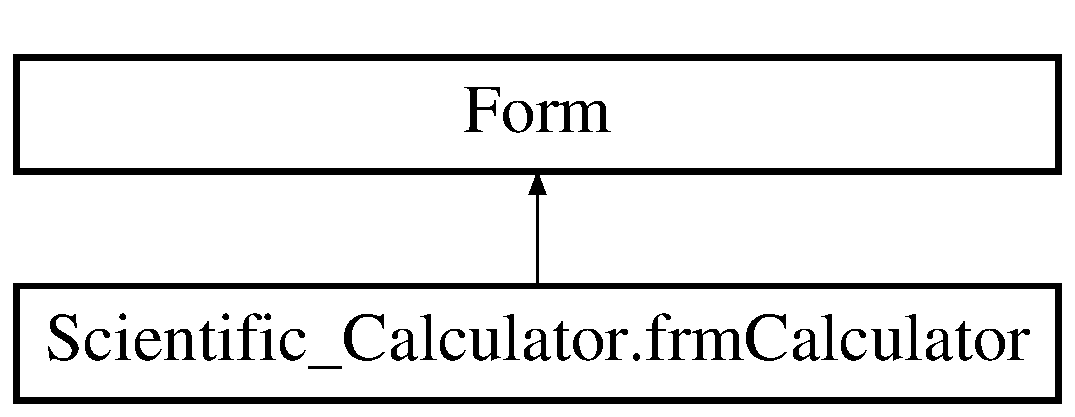
\includegraphics[height=2.000000cm]{class_scientific___calculator_1_1frm_calculator}
\end{center}
\end{figure}
\subsection*{Public Member Functions}
\begin{DoxyCompactItemize}
\item 
\hyperlink{class_scientific___calculator_1_1frm_calculator_a0959073ecdf7a5b1f1bee0b47a56cee9}{frm\+Calculator} ()
\begin{DoxyCompactList}\small\item\em Constructor \end{DoxyCompactList}\end{DoxyCompactItemize}
\subsection*{Protected Member Functions}
\begin{DoxyCompactItemize}
\item 
override void \hyperlink{class_scientific___calculator_1_1frm_calculator_a3839d5570f4cf4bf018fbed788f93823}{Dispose} (bool disposing)
\begin{DoxyCompactList}\small\item\em Clean up any resources being used. \end{DoxyCompactList}\end{DoxyCompactItemize}


\subsection{Detailed Description}
Main form, contains the calculator itself and buttons to open all the other forms as dialog windows 



\subsection{Constructor \& Destructor Documentation}
\mbox{\Hypertarget{class_scientific___calculator_1_1frm_calculator_a0959073ecdf7a5b1f1bee0b47a56cee9}\label{class_scientific___calculator_1_1frm_calculator_a0959073ecdf7a5b1f1bee0b47a56cee9}} 
\index{Scientific\+\_\+\+Calculator\+::frm\+Calculator@{Scientific\+\_\+\+Calculator\+::frm\+Calculator}!frm\+Calculator@{frm\+Calculator}}
\index{frm\+Calculator@{frm\+Calculator}!Scientific\+\_\+\+Calculator\+::frm\+Calculator@{Scientific\+\_\+\+Calculator\+::frm\+Calculator}}
\subsubsection{\texorpdfstring{frm\+Calculator()}{frmCalculator()}}
{\footnotesize\ttfamily Scientific\+\_\+\+Calculator.\+frm\+Calculator.\+frm\+Calculator (\begin{DoxyParamCaption}{ }\end{DoxyParamCaption})}



Constructor 



\subsection{Member Function Documentation}
\mbox{\Hypertarget{class_scientific___calculator_1_1frm_calculator_a3839d5570f4cf4bf018fbed788f93823}\label{class_scientific___calculator_1_1frm_calculator_a3839d5570f4cf4bf018fbed788f93823}} 
\index{Scientific\+\_\+\+Calculator\+::frm\+Calculator@{Scientific\+\_\+\+Calculator\+::frm\+Calculator}!Dispose@{Dispose}}
\index{Dispose@{Dispose}!Scientific\+\_\+\+Calculator\+::frm\+Calculator@{Scientific\+\_\+\+Calculator\+::frm\+Calculator}}
\subsubsection{\texorpdfstring{Dispose()}{Dispose()}}
{\footnotesize\ttfamily override void Scientific\+\_\+\+Calculator.\+frm\+Calculator.\+Dispose (\begin{DoxyParamCaption}\item[{bool}]{disposing }\end{DoxyParamCaption})\hspace{0.3cm}{\ttfamily [protected]}}



Clean up any resources being used. 


\begin{DoxyParams}{Parameters}
{\em disposing} & true if managed resources should be disposed; otherwise, false.\\
\hline
\end{DoxyParams}


The documentation for this class was generated from the following files\+:\begin{DoxyCompactItemize}
\item 
C\+:/\+Scientific\+\_\+\+Calculator/\+Scientific\+\_\+\+Calculator/\+Code/\+Scientific\+\_\+\+Calculator/\+Scientific\+\_\+\+Calculator/\hyperlink{frm_calculator_8cs}{frm\+Calculator.\+cs}\item 
C\+:/\+Scientific\+\_\+\+Calculator/\+Scientific\+\_\+\+Calculator/\+Code/\+Scientific\+\_\+\+Calculator/\+Scientific\+\_\+\+Calculator/\hyperlink{frm_calculator_8_designer_8cs}{frm\+Calculator.\+Designer.\+cs}\end{DoxyCompactItemize}

\hypertarget{class_scientific___calculator_1_1frm_function_plot}{}\section{Scientific\+\_\+\+Calculator.\+frm\+Function\+Plot Class Reference}
\label{class_scientific___calculator_1_1frm_function_plot}\index{Scientific\+\_\+\+Calculator.\+frm\+Function\+Plot@{Scientific\+\_\+\+Calculator.\+frm\+Function\+Plot}}


Form that displays a graph from a given function  


Inheritance diagram for Scientific\+\_\+\+Calculator.\+frm\+Function\+Plot\+:\begin{figure}[H]
\begin{center}
\leavevmode
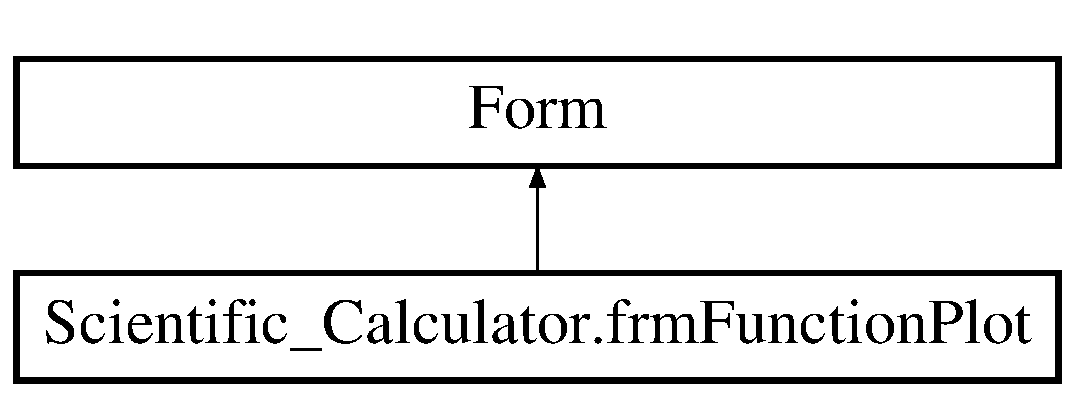
\includegraphics[height=2.000000cm]{class_scientific___calculator_1_1frm_function_plot}
\end{center}
\end{figure}
\subsection*{Public Member Functions}
\begin{DoxyCompactItemize}
\item 
\hyperlink{class_scientific___calculator_1_1frm_function_plot_ae747a0991aecf3c9f82e111913248f1a}{frm\+Function\+Plot} ()
\begin{DoxyCompactList}\small\item\em Constructor \end{DoxyCompactList}\end{DoxyCompactItemize}
\subsection*{Protected Member Functions}
\begin{DoxyCompactItemize}
\item 
override void \hyperlink{class_scientific___calculator_1_1frm_function_plot_aa502a35dc8fc827e93659199df349dce}{Dispose} (bool disposing)
\begin{DoxyCompactList}\small\item\em Clean up any resources being used. \end{DoxyCompactList}\end{DoxyCompactItemize}


\subsection{Detailed Description}
Form that displays a graph from a given function 



\subsection{Constructor \& Destructor Documentation}
\mbox{\Hypertarget{class_scientific___calculator_1_1frm_function_plot_ae747a0991aecf3c9f82e111913248f1a}\label{class_scientific___calculator_1_1frm_function_plot_ae747a0991aecf3c9f82e111913248f1a}} 
\index{Scientific\+\_\+\+Calculator\+::frm\+Function\+Plot@{Scientific\+\_\+\+Calculator\+::frm\+Function\+Plot}!frm\+Function\+Plot@{frm\+Function\+Plot}}
\index{frm\+Function\+Plot@{frm\+Function\+Plot}!Scientific\+\_\+\+Calculator\+::frm\+Function\+Plot@{Scientific\+\_\+\+Calculator\+::frm\+Function\+Plot}}
\subsubsection{\texorpdfstring{frm\+Function\+Plot()}{frmFunctionPlot()}}
{\footnotesize\ttfamily Scientific\+\_\+\+Calculator.\+frm\+Function\+Plot.\+frm\+Function\+Plot (\begin{DoxyParamCaption}{ }\end{DoxyParamCaption})}



Constructor 



\subsection{Member Function Documentation}
\mbox{\Hypertarget{class_scientific___calculator_1_1frm_function_plot_aa502a35dc8fc827e93659199df349dce}\label{class_scientific___calculator_1_1frm_function_plot_aa502a35dc8fc827e93659199df349dce}} 
\index{Scientific\+\_\+\+Calculator\+::frm\+Function\+Plot@{Scientific\+\_\+\+Calculator\+::frm\+Function\+Plot}!Dispose@{Dispose}}
\index{Dispose@{Dispose}!Scientific\+\_\+\+Calculator\+::frm\+Function\+Plot@{Scientific\+\_\+\+Calculator\+::frm\+Function\+Plot}}
\subsubsection{\texorpdfstring{Dispose()}{Dispose()}}
{\footnotesize\ttfamily override void Scientific\+\_\+\+Calculator.\+frm\+Function\+Plot.\+Dispose (\begin{DoxyParamCaption}\item[{bool}]{disposing }\end{DoxyParamCaption})\hspace{0.3cm}{\ttfamily [protected]}}



Clean up any resources being used. 


\begin{DoxyParams}{Parameters}
{\em disposing} & true if managed resources should be disposed; otherwise, false.\\
\hline
\end{DoxyParams}


The documentation for this class was generated from the following files\+:\begin{DoxyCompactItemize}
\item 
C\+:/\+Scientific\+\_\+\+Calculator/\+Scientific\+\_\+\+Calculator/\+Code/\+Scientific\+\_\+\+Calculator/\+Scientific\+\_\+\+Calculator/\hyperlink{frm_function_plot_8cs}{frm\+Function\+Plot.\+cs}\item 
C\+:/\+Scientific\+\_\+\+Calculator/\+Scientific\+\_\+\+Calculator/\+Code/\+Scientific\+\_\+\+Calculator/\+Scientific\+\_\+\+Calculator/\hyperlink{frm_function_plot_8_designer_8cs}{frm\+Function\+Plot.\+Designer.\+cs}\end{DoxyCompactItemize}

\hypertarget{class_scientific___calculator_1_1frm_history}{}\section{Scientific\+\_\+\+Calculator.\+frm\+History Class Reference}
\label{class_scientific___calculator_1_1frm_history}\index{Scientific\+\_\+\+Calculator.\+frm\+History@{Scientific\+\_\+\+Calculator.\+frm\+History}}


Form that displays the operations history on a listbox  


Inheritance diagram for Scientific\+\_\+\+Calculator.\+frm\+History\+:\begin{figure}[H]
\begin{center}
\leavevmode
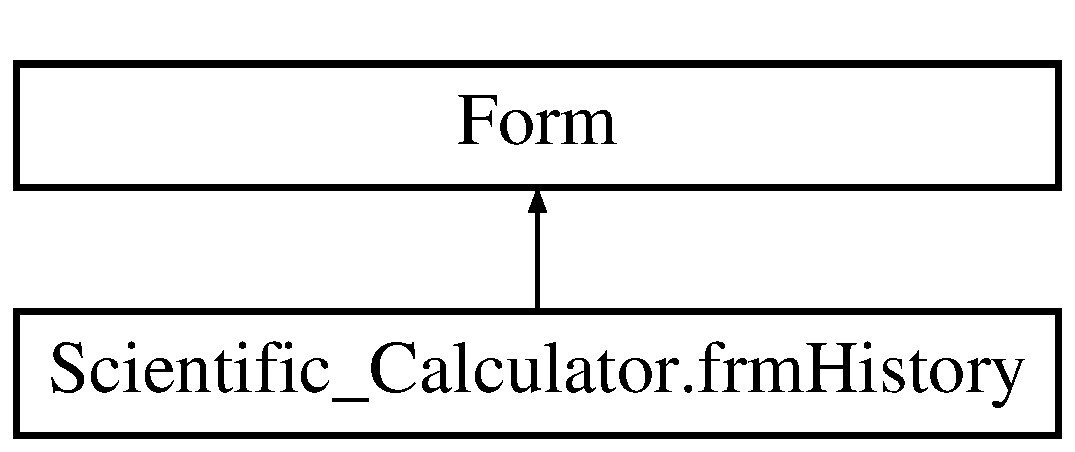
\includegraphics[height=2.000000cm]{class_scientific___calculator_1_1frm_history}
\end{center}
\end{figure}
\subsection*{Public Member Functions}
\begin{DoxyCompactItemize}
\item 
\hyperlink{class_scientific___calculator_1_1frm_history_aab640c35614c8ad1c64b1e3150bd8ed1}{frm\+History} ()
\begin{DoxyCompactList}\small\item\em Constructor. Calls the Display\+History method when finished. \end{DoxyCompactList}\end{DoxyCompactItemize}
\subsection*{Protected Member Functions}
\begin{DoxyCompactItemize}
\item 
override void \hyperlink{class_scientific___calculator_1_1frm_history_adf91a5ec5e4df47f129c8a1a57161155}{Dispose} (bool disposing)
\begin{DoxyCompactList}\small\item\em Clean up any resources being used. \end{DoxyCompactList}\end{DoxyCompactItemize}


\subsection{Detailed Description}
Form that displays the operations history on a listbox 



\subsection{Constructor \& Destructor Documentation}
\mbox{\Hypertarget{class_scientific___calculator_1_1frm_history_aab640c35614c8ad1c64b1e3150bd8ed1}\label{class_scientific___calculator_1_1frm_history_aab640c35614c8ad1c64b1e3150bd8ed1}} 
\index{Scientific\+\_\+\+Calculator\+::frm\+History@{Scientific\+\_\+\+Calculator\+::frm\+History}!frm\+History@{frm\+History}}
\index{frm\+History@{frm\+History}!Scientific\+\_\+\+Calculator\+::frm\+History@{Scientific\+\_\+\+Calculator\+::frm\+History}}
\subsubsection{\texorpdfstring{frm\+History()}{frmHistory()}}
{\footnotesize\ttfamily Scientific\+\_\+\+Calculator.\+frm\+History.\+frm\+History (\begin{DoxyParamCaption}{ }\end{DoxyParamCaption})}



Constructor. Calls the Display\+History method when finished. 



\subsection{Member Function Documentation}
\mbox{\Hypertarget{class_scientific___calculator_1_1frm_history_adf91a5ec5e4df47f129c8a1a57161155}\label{class_scientific___calculator_1_1frm_history_adf91a5ec5e4df47f129c8a1a57161155}} 
\index{Scientific\+\_\+\+Calculator\+::frm\+History@{Scientific\+\_\+\+Calculator\+::frm\+History}!Dispose@{Dispose}}
\index{Dispose@{Dispose}!Scientific\+\_\+\+Calculator\+::frm\+History@{Scientific\+\_\+\+Calculator\+::frm\+History}}
\subsubsection{\texorpdfstring{Dispose()}{Dispose()}}
{\footnotesize\ttfamily override void Scientific\+\_\+\+Calculator.\+frm\+History.\+Dispose (\begin{DoxyParamCaption}\item[{bool}]{disposing }\end{DoxyParamCaption})\hspace{0.3cm}{\ttfamily [protected]}}



Clean up any resources being used. 


\begin{DoxyParams}{Parameters}
{\em disposing} & true if managed resources should be disposed; otherwise, false.\\
\hline
\end{DoxyParams}


The documentation for this class was generated from the following files\+:\begin{DoxyCompactItemize}
\item 
C\+:/\+Scientific\+\_\+\+Calculator/\+Scientific\+\_\+\+Calculator/\+Code/\+Scientific\+\_\+\+Calculator/\+Scientific\+\_\+\+Calculator/\hyperlink{frm_history_8cs}{frm\+History.\+cs}\item 
C\+:/\+Scientific\+\_\+\+Calculator/\+Scientific\+\_\+\+Calculator/\+Code/\+Scientific\+\_\+\+Calculator/\+Scientific\+\_\+\+Calculator/\hyperlink{frm_history_8_designer_8cs}{frm\+History.\+Designer.\+cs}\end{DoxyCompactItemize}

\hypertarget{class_scientific___calculator_1_1frm_settings}{}\section{Scientific\+\_\+\+Calculator.\+frm\+Settings Class Reference}
\label{class_scientific___calculator_1_1frm_settings}\index{Scientific\+\_\+\+Calculator.\+frm\+Settings@{Scientific\+\_\+\+Calculator.\+frm\+Settings}}


Form that allows the user to change some application settings  


Inheritance diagram for Scientific\+\_\+\+Calculator.\+frm\+Settings\+:\begin{figure}[H]
\begin{center}
\leavevmode
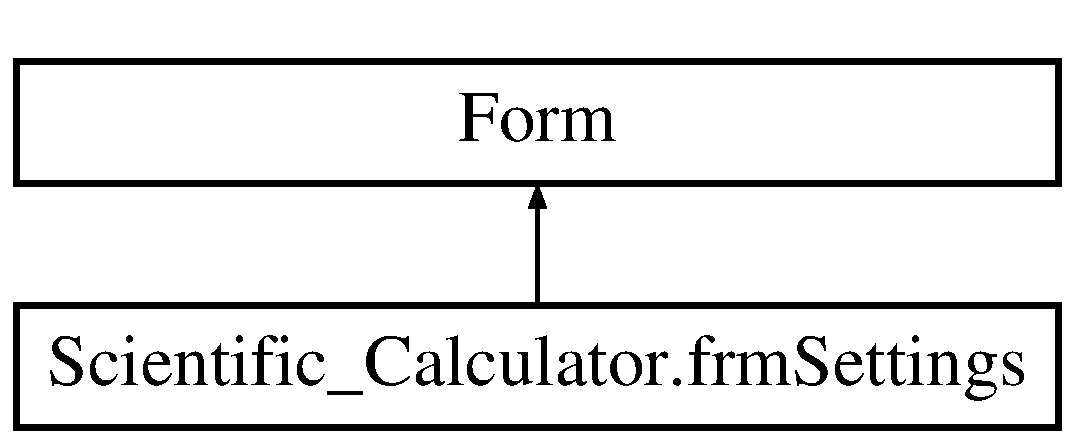
\includegraphics[height=2.000000cm]{class_scientific___calculator_1_1frm_settings}
\end{center}
\end{figure}
\subsection*{Public Member Functions}
\begin{DoxyCompactItemize}
\item 
\hyperlink{class_scientific___calculator_1_1frm_settings_a240b88000ca34b6a5e34b560e5e32f20}{frm\+Settings} ()
\begin{DoxyCompactList}\small\item\em Constructor \end{DoxyCompactList}\end{DoxyCompactItemize}
\subsection*{Protected Member Functions}
\begin{DoxyCompactItemize}
\item 
override void \hyperlink{class_scientific___calculator_1_1frm_settings_a3f5e63317d8fef66f6587a1a19b21b44}{Dispose} (bool disposing)
\begin{DoxyCompactList}\small\item\em Clean up any resources being used. \end{DoxyCompactList}\end{DoxyCompactItemize}


\subsection{Detailed Description}
Form that allows the user to change some application settings 



\subsection{Constructor \& Destructor Documentation}
\mbox{\Hypertarget{class_scientific___calculator_1_1frm_settings_a240b88000ca34b6a5e34b560e5e32f20}\label{class_scientific___calculator_1_1frm_settings_a240b88000ca34b6a5e34b560e5e32f20}} 
\index{Scientific\+\_\+\+Calculator\+::frm\+Settings@{Scientific\+\_\+\+Calculator\+::frm\+Settings}!frm\+Settings@{frm\+Settings}}
\index{frm\+Settings@{frm\+Settings}!Scientific\+\_\+\+Calculator\+::frm\+Settings@{Scientific\+\_\+\+Calculator\+::frm\+Settings}}
\subsubsection{\texorpdfstring{frm\+Settings()}{frmSettings()}}
{\footnotesize\ttfamily Scientific\+\_\+\+Calculator.\+frm\+Settings.\+frm\+Settings (\begin{DoxyParamCaption}{ }\end{DoxyParamCaption})}



Constructor 



\subsection{Member Function Documentation}
\mbox{\Hypertarget{class_scientific___calculator_1_1frm_settings_a3f5e63317d8fef66f6587a1a19b21b44}\label{class_scientific___calculator_1_1frm_settings_a3f5e63317d8fef66f6587a1a19b21b44}} 
\index{Scientific\+\_\+\+Calculator\+::frm\+Settings@{Scientific\+\_\+\+Calculator\+::frm\+Settings}!Dispose@{Dispose}}
\index{Dispose@{Dispose}!Scientific\+\_\+\+Calculator\+::frm\+Settings@{Scientific\+\_\+\+Calculator\+::frm\+Settings}}
\subsubsection{\texorpdfstring{Dispose()}{Dispose()}}
{\footnotesize\ttfamily override void Scientific\+\_\+\+Calculator.\+frm\+Settings.\+Dispose (\begin{DoxyParamCaption}\item[{bool}]{disposing }\end{DoxyParamCaption})\hspace{0.3cm}{\ttfamily [protected]}}



Clean up any resources being used. 


\begin{DoxyParams}{Parameters}
{\em disposing} & true if managed resources should be disposed; otherwise, false.\\
\hline
\end{DoxyParams}


The documentation for this class was generated from the following files\+:\begin{DoxyCompactItemize}
\item 
C\+:/\+Scientific\+\_\+\+Calculator/\+Scientific\+\_\+\+Calculator/\+Code/\+Scientific\+\_\+\+Calculator/\+Scientific\+\_\+\+Calculator/\hyperlink{frm_settings_8cs}{frm\+Settings.\+cs}\item 
C\+:/\+Scientific\+\_\+\+Calculator/\+Scientific\+\_\+\+Calculator/\+Code/\+Scientific\+\_\+\+Calculator/\+Scientific\+\_\+\+Calculator/\hyperlink{frm_settings_8_designer_8cs}{frm\+Settings.\+Designer.\+cs}\end{DoxyCompactItemize}

\chapter{File Documentation}
\hypertarget{_calculation_8cs}{}\section{C\+:/\+Scientific\+\_\+\+Calculator/\+Scientific\+\_\+\+Calculator/\+Code/\+Scientific\+\_\+\+Calculator/\+Scientific\+\_\+\+Calculator/\+Calculation.cs File Reference}
\label{_calculation_8cs}\index{C\+:/\+Scientific\+\_\+\+Calculator/\+Scientific\+\_\+\+Calculator/\+Code/\+Scientific\+\_\+\+Calculator/\+Scientific\+\_\+\+Calculator/\+Calculation.\+cs@{C\+:/\+Scientific\+\_\+\+Calculator/\+Scientific\+\_\+\+Calculator/\+Code/\+Scientific\+\_\+\+Calculator/\+Scientific\+\_\+\+Calculator/\+Calculation.\+cs}}
\subsection*{Classes}
\begin{DoxyCompactItemize}
\item 
class \hyperlink{class_scientific___calculator_1_1_calculation}{Scientific\+\_\+\+Calculator.\+Calculation}
\begin{DoxyCompactList}\small\item\em Class that handles all the mathematics of the program, and interpretes the operations inputs \end{DoxyCompactList}\end{DoxyCompactItemize}
\subsection*{Namespaces}
\begin{DoxyCompactItemize}
\item 
namespace \hyperlink{namespace_scientific___calculator}{Scientific\+\_\+\+Calculator}
\end{DoxyCompactItemize}

\hypertarget{_d_b_access_8cs}{}\section{C\+:/\+Scientific\+\_\+\+Calculator/\+Scientific\+\_\+\+Calculator/\+Code/\+Scientific\+\_\+\+Calculator/\+Scientific\+\_\+\+Calculator/\+D\+B\+Access.cs File Reference}
\label{_d_b_access_8cs}\index{C\+:/\+Scientific\+\_\+\+Calculator/\+Scientific\+\_\+\+Calculator/\+Code/\+Scientific\+\_\+\+Calculator/\+Scientific\+\_\+\+Calculator/\+D\+B\+Access.\+cs@{C\+:/\+Scientific\+\_\+\+Calculator/\+Scientific\+\_\+\+Calculator/\+Code/\+Scientific\+\_\+\+Calculator/\+Scientific\+\_\+\+Calculator/\+D\+B\+Access.\+cs}}
\subsection*{Classes}
\begin{DoxyCompactItemize}
\item 
class \hyperlink{class_scientific___calculator_1_1_d_b_access}{Scientific\+\_\+\+Calculator.\+D\+B\+Access}
\begin{DoxyCompactList}\small\item\em Class that handles all the database operations \end{DoxyCompactList}\end{DoxyCompactItemize}
\subsection*{Namespaces}
\begin{DoxyCompactItemize}
\item 
namespace \hyperlink{namespace_scientific___calculator}{Scientific\+\_\+\+Calculator}
\end{DoxyCompactItemize}

\hypertarget{frm_calculator_8cs}{}\section{C\+:/\+Scientific\+\_\+\+Calculator/\+Scientific\+\_\+\+Calculator/\+Code/\+Scientific\+\_\+\+Calculator/\+Scientific\+\_\+\+Calculator/frm\+Calculator.cs File Reference}
\label{frm_calculator_8cs}\index{C\+:/\+Scientific\+\_\+\+Calculator/\+Scientific\+\_\+\+Calculator/\+Code/\+Scientific\+\_\+\+Calculator/\+Scientific\+\_\+\+Calculator/frm\+Calculator.\+cs@{C\+:/\+Scientific\+\_\+\+Calculator/\+Scientific\+\_\+\+Calculator/\+Code/\+Scientific\+\_\+\+Calculator/\+Scientific\+\_\+\+Calculator/frm\+Calculator.\+cs}}
\subsection*{Classes}
\begin{DoxyCompactItemize}
\item 
class \hyperlink{class_scientific___calculator_1_1frm_calculator}{Scientific\+\_\+\+Calculator.\+frm\+Calculator}
\begin{DoxyCompactList}\small\item\em Main form, contains the calculator itself and buttons to open all the other forms as dialog windows \end{DoxyCompactList}\end{DoxyCompactItemize}
\subsection*{Namespaces}
\begin{DoxyCompactItemize}
\item 
namespace \hyperlink{namespace_scientific___calculator}{Scientific\+\_\+\+Calculator}
\end{DoxyCompactItemize}

\hypertarget{frm_calculator_8_designer_8cs}{}\section{C\+:/\+Scientific\+\_\+\+Calculator/\+Scientific\+\_\+\+Calculator/\+Code/\+Scientific\+\_\+\+Calculator/\+Scientific\+\_\+\+Calculator/frm\+Calculator.Designer.\+cs File Reference}
\label{frm_calculator_8_designer_8cs}\index{C\+:/\+Scientific\+\_\+\+Calculator/\+Scientific\+\_\+\+Calculator/\+Code/\+Scientific\+\_\+\+Calculator/\+Scientific\+\_\+\+Calculator/frm\+Calculator.\+Designer.\+cs@{C\+:/\+Scientific\+\_\+\+Calculator/\+Scientific\+\_\+\+Calculator/\+Code/\+Scientific\+\_\+\+Calculator/\+Scientific\+\_\+\+Calculator/frm\+Calculator.\+Designer.\+cs}}
\subsection*{Classes}
\begin{DoxyCompactItemize}
\item 
class \hyperlink{class_scientific___calculator_1_1frm_calculator}{Scientific\+\_\+\+Calculator.\+frm\+Calculator}
\begin{DoxyCompactList}\small\item\em Main form, contains the calculator itself and buttons to open all the other forms as dialog windows \end{DoxyCompactList}\end{DoxyCompactItemize}
\subsection*{Namespaces}
\begin{DoxyCompactItemize}
\item 
namespace \hyperlink{namespace_scientific___calculator}{Scientific\+\_\+\+Calculator}
\end{DoxyCompactItemize}

\hypertarget{frm_function_plot_8cs}{}\section{C\+:/\+Scientific\+\_\+\+Calculator/\+Scientific\+\_\+\+Calculator/\+Code/\+Scientific\+\_\+\+Calculator/\+Scientific\+\_\+\+Calculator/frm\+Function\+Plot.cs File Reference}
\label{frm_function_plot_8cs}\index{C\+:/\+Scientific\+\_\+\+Calculator/\+Scientific\+\_\+\+Calculator/\+Code/\+Scientific\+\_\+\+Calculator/\+Scientific\+\_\+\+Calculator/frm\+Function\+Plot.\+cs@{C\+:/\+Scientific\+\_\+\+Calculator/\+Scientific\+\_\+\+Calculator/\+Code/\+Scientific\+\_\+\+Calculator/\+Scientific\+\_\+\+Calculator/frm\+Function\+Plot.\+cs}}
\subsection*{Classes}
\begin{DoxyCompactItemize}
\item 
class \hyperlink{class_scientific___calculator_1_1frm_function_plot}{Scientific\+\_\+\+Calculator.\+frm\+Function\+Plot}
\begin{DoxyCompactList}\small\item\em Form that displays a graph from a given function \end{DoxyCompactList}\end{DoxyCompactItemize}
\subsection*{Namespaces}
\begin{DoxyCompactItemize}
\item 
namespace \hyperlink{namespace_scientific___calculator}{Scientific\+\_\+\+Calculator}
\end{DoxyCompactItemize}

\hypertarget{frm_function_plot_8_designer_8cs}{}\section{C\+:/\+Scientific\+\_\+\+Calculator/\+Scientific\+\_\+\+Calculator/\+Code/\+Scientific\+\_\+\+Calculator/\+Scientific\+\_\+\+Calculator/frm\+Function\+Plot.Designer.\+cs File Reference}
\label{frm_function_plot_8_designer_8cs}\index{C\+:/\+Scientific\+\_\+\+Calculator/\+Scientific\+\_\+\+Calculator/\+Code/\+Scientific\+\_\+\+Calculator/\+Scientific\+\_\+\+Calculator/frm\+Function\+Plot.\+Designer.\+cs@{C\+:/\+Scientific\+\_\+\+Calculator/\+Scientific\+\_\+\+Calculator/\+Code/\+Scientific\+\_\+\+Calculator/\+Scientific\+\_\+\+Calculator/frm\+Function\+Plot.\+Designer.\+cs}}
\subsection*{Classes}
\begin{DoxyCompactItemize}
\item 
class \hyperlink{class_scientific___calculator_1_1frm_function_plot}{Scientific\+\_\+\+Calculator.\+frm\+Function\+Plot}
\begin{DoxyCompactList}\small\item\em Form that displays a graph from a given function \end{DoxyCompactList}\end{DoxyCompactItemize}
\subsection*{Namespaces}
\begin{DoxyCompactItemize}
\item 
namespace \hyperlink{namespace_scientific___calculator}{Scientific\+\_\+\+Calculator}
\end{DoxyCompactItemize}

\hypertarget{frm_history_8cs}{}\section{C\+:/\+Scientific\+\_\+\+Calculator/\+Scientific\+\_\+\+Calculator/\+Code/\+Scientific\+\_\+\+Calculator/\+Scientific\+\_\+\+Calculator/frm\+History.cs File Reference}
\label{frm_history_8cs}\index{C\+:/\+Scientific\+\_\+\+Calculator/\+Scientific\+\_\+\+Calculator/\+Code/\+Scientific\+\_\+\+Calculator/\+Scientific\+\_\+\+Calculator/frm\+History.\+cs@{C\+:/\+Scientific\+\_\+\+Calculator/\+Scientific\+\_\+\+Calculator/\+Code/\+Scientific\+\_\+\+Calculator/\+Scientific\+\_\+\+Calculator/frm\+History.\+cs}}
\subsection*{Classes}
\begin{DoxyCompactItemize}
\item 
class \hyperlink{class_scientific___calculator_1_1frm_history}{Scientific\+\_\+\+Calculator.\+frm\+History}
\begin{DoxyCompactList}\small\item\em Form that displays the operations history on a listbox \end{DoxyCompactList}\end{DoxyCompactItemize}
\subsection*{Namespaces}
\begin{DoxyCompactItemize}
\item 
namespace \hyperlink{namespace_scientific___calculator}{Scientific\+\_\+\+Calculator}
\end{DoxyCompactItemize}

\hypertarget{frm_history_8_designer_8cs}{}\section{C\+:/\+Scientific\+\_\+\+Calculator/\+Scientific\+\_\+\+Calculator/\+Code/\+Scientific\+\_\+\+Calculator/\+Scientific\+\_\+\+Calculator/frm\+History.Designer.\+cs File Reference}
\label{frm_history_8_designer_8cs}\index{C\+:/\+Scientific\+\_\+\+Calculator/\+Scientific\+\_\+\+Calculator/\+Code/\+Scientific\+\_\+\+Calculator/\+Scientific\+\_\+\+Calculator/frm\+History.\+Designer.\+cs@{C\+:/\+Scientific\+\_\+\+Calculator/\+Scientific\+\_\+\+Calculator/\+Code/\+Scientific\+\_\+\+Calculator/\+Scientific\+\_\+\+Calculator/frm\+History.\+Designer.\+cs}}
\subsection*{Classes}
\begin{DoxyCompactItemize}
\item 
class \hyperlink{class_scientific___calculator_1_1frm_history}{Scientific\+\_\+\+Calculator.\+frm\+History}
\begin{DoxyCompactList}\small\item\em Form that displays the operations history on a listbox \end{DoxyCompactList}\end{DoxyCompactItemize}
\subsection*{Namespaces}
\begin{DoxyCompactItemize}
\item 
namespace \hyperlink{namespace_scientific___calculator}{Scientific\+\_\+\+Calculator}
\end{DoxyCompactItemize}

\hypertarget{frm_settings_8cs}{}\section{C\+:/\+Scientific\+\_\+\+Calculator/\+Scientific\+\_\+\+Calculator/\+Code/\+Scientific\+\_\+\+Calculator/\+Scientific\+\_\+\+Calculator/frm\+Settings.cs File Reference}
\label{frm_settings_8cs}\index{C\+:/\+Scientific\+\_\+\+Calculator/\+Scientific\+\_\+\+Calculator/\+Code/\+Scientific\+\_\+\+Calculator/\+Scientific\+\_\+\+Calculator/frm\+Settings.\+cs@{C\+:/\+Scientific\+\_\+\+Calculator/\+Scientific\+\_\+\+Calculator/\+Code/\+Scientific\+\_\+\+Calculator/\+Scientific\+\_\+\+Calculator/frm\+Settings.\+cs}}
\subsection*{Classes}
\begin{DoxyCompactItemize}
\item 
class \hyperlink{class_scientific___calculator_1_1frm_settings}{Scientific\+\_\+\+Calculator.\+frm\+Settings}
\begin{DoxyCompactList}\small\item\em Form that allows the user to change some application settings \end{DoxyCompactList}\end{DoxyCompactItemize}
\subsection*{Namespaces}
\begin{DoxyCompactItemize}
\item 
namespace \hyperlink{namespace_scientific___calculator}{Scientific\+\_\+\+Calculator}
\end{DoxyCompactItemize}

\hypertarget{frm_settings_8_designer_8cs}{}\section{C\+:/\+Scientific\+\_\+\+Calculator/\+Scientific\+\_\+\+Calculator/\+Code/\+Scientific\+\_\+\+Calculator/\+Scientific\+\_\+\+Calculator/frm\+Settings.Designer.\+cs File Reference}
\label{frm_settings_8_designer_8cs}\index{C\+:/\+Scientific\+\_\+\+Calculator/\+Scientific\+\_\+\+Calculator/\+Code/\+Scientific\+\_\+\+Calculator/\+Scientific\+\_\+\+Calculator/frm\+Settings.\+Designer.\+cs@{C\+:/\+Scientific\+\_\+\+Calculator/\+Scientific\+\_\+\+Calculator/\+Code/\+Scientific\+\_\+\+Calculator/\+Scientific\+\_\+\+Calculator/frm\+Settings.\+Designer.\+cs}}
\subsection*{Classes}
\begin{DoxyCompactItemize}
\item 
class \hyperlink{class_scientific___calculator_1_1frm_settings}{Scientific\+\_\+\+Calculator.\+frm\+Settings}
\begin{DoxyCompactList}\small\item\em Form that allows the user to change some application settings \end{DoxyCompactList}\end{DoxyCompactItemize}
\subsection*{Namespaces}
\begin{DoxyCompactItemize}
\item 
namespace \hyperlink{namespace_scientific___calculator}{Scientific\+\_\+\+Calculator}
\end{DoxyCompactItemize}

\hypertarget{_temporary_generated_file__036_c0_b5_b-1481-4323-8_d20-8_f5_a_d_c_b23_d92_8cs}{}\section{C\+:/\+Scientific\+\_\+\+Calculator/\+Scientific\+\_\+\+Calculator/\+Code/\+Scientific\+\_\+\+Calculator/\+Scientific\+\_\+\+Calculator/obj/\+Debug/\+Temporary\+Generated\+File\+\_\+036\+C0\+B5\+B-\/1481-\/4323-\/8\+D20-\/8\+F5\+A\+D\+C\+B23\+D92.cs File Reference}
\label{_temporary_generated_file__036_c0_b5_b-1481-4323-8_d20-8_f5_a_d_c_b23_d92_8cs}\index{C\+:/\+Scientific\+\_\+\+Calculator/\+Scientific\+\_\+\+Calculator/\+Code/\+Scientific\+\_\+\+Calculator/\+Scientific\+\_\+\+Calculator/obj/\+Debug/\+Temporary\+Generated\+File\+\_\+036\+C0\+B5\+B-\/1481-\/4323-\/8\+D20-\/8\+F5\+A\+D\+C\+B23\+D92.\+cs@{C\+:/\+Scientific\+\_\+\+Calculator/\+Scientific\+\_\+\+Calculator/\+Code/\+Scientific\+\_\+\+Calculator/\+Scientific\+\_\+\+Calculator/obj/\+Debug/\+Temporary\+Generated\+File\+\_\+036\+C0\+B5\+B-\/1481-\/4323-\/8\+D20-\/8\+F5\+A\+D\+C\+B23\+D92.\+cs}}

\hypertarget{_temporary_generated_file__5937a670-0e60-4077-877b-f7221da3dda1_8cs}{}\section{C\+:/\+Scientific\+\_\+\+Calculator/\+Scientific\+\_\+\+Calculator/\+Code/\+Scientific\+\_\+\+Calculator/\+Scientific\+\_\+\+Calculator/obj/\+Debug/\+Temporary\+Generated\+File\+\_\+5937a670-\/0e60-\/4077-\/877b-\/f7221da3dda1.cs File Reference}
\label{_temporary_generated_file__5937a670-0e60-4077-877b-f7221da3dda1_8cs}\index{C\+:/\+Scientific\+\_\+\+Calculator/\+Scientific\+\_\+\+Calculator/\+Code/\+Scientific\+\_\+\+Calculator/\+Scientific\+\_\+\+Calculator/obj/\+Debug/\+Temporary\+Generated\+File\+\_\+5937a670-\/0e60-\/4077-\/877b-\/f7221da3dda1.\+cs@{C\+:/\+Scientific\+\_\+\+Calculator/\+Scientific\+\_\+\+Calculator/\+Code/\+Scientific\+\_\+\+Calculator/\+Scientific\+\_\+\+Calculator/obj/\+Debug/\+Temporary\+Generated\+File\+\_\+5937a670-\/0e60-\/4077-\/877b-\/f7221da3dda1.\+cs}}

\hypertarget{_temporary_generated_file___e7_a71_f73-0_f8_d-4_b9_b-_b56_e-8_e70_b10_b_c5_d3_8cs}{}\section{C\+:/\+Scientific\+\_\+\+Calculator/\+Scientific\+\_\+\+Calculator/\+Code/\+Scientific\+\_\+\+Calculator/\+Scientific\+\_\+\+Calculator/obj/\+Debug/\+Temporary\+Generated\+File\+\_\+\+E7\+A71\+F73-\/0\+F8\+D-\/4\+B9\+B-\/\+B56\+E-\/8\+E70\+B10\+B\+C5\+D3.cs File Reference}
\label{_temporary_generated_file___e7_a71_f73-0_f8_d-4_b9_b-_b56_e-8_e70_b10_b_c5_d3_8cs}\index{C\+:/\+Scientific\+\_\+\+Calculator/\+Scientific\+\_\+\+Calculator/\+Code/\+Scientific\+\_\+\+Calculator/\+Scientific\+\_\+\+Calculator/obj/\+Debug/\+Temporary\+Generated\+File\+\_\+\+E7\+A71\+F73-\/0\+F8\+D-\/4\+B9\+B-\/\+B56\+E-\/8\+E70\+B10\+B\+C5\+D3.\+cs@{C\+:/\+Scientific\+\_\+\+Calculator/\+Scientific\+\_\+\+Calculator/\+Code/\+Scientific\+\_\+\+Calculator/\+Scientific\+\_\+\+Calculator/obj/\+Debug/\+Temporary\+Generated\+File\+\_\+\+E7\+A71\+F73-\/0\+F8\+D-\/4\+B9\+B-\/\+B56\+E-\/8\+E70\+B10\+B\+C5\+D3.\+cs}}

\hypertarget{_program_8cs}{}\section{C\+:/\+Scientific\+\_\+\+Calculator/\+Scientific\+\_\+\+Calculator/\+Code/\+Scientific\+\_\+\+Calculator/\+Scientific\+\_\+\+Calculator/\+Program.cs File Reference}
\label{_program_8cs}\index{C\+:/\+Scientific\+\_\+\+Calculator/\+Scientific\+\_\+\+Calculator/\+Code/\+Scientific\+\_\+\+Calculator/\+Scientific\+\_\+\+Calculator/\+Program.\+cs@{C\+:/\+Scientific\+\_\+\+Calculator/\+Scientific\+\_\+\+Calculator/\+Code/\+Scientific\+\_\+\+Calculator/\+Scientific\+\_\+\+Calculator/\+Program.\+cs}}
\subsection*{Classes}
\begin{DoxyCompactItemize}
\item 
class {\bfseries Scientific\+\_\+\+Calculator.\+Program}
\end{DoxyCompactItemize}
\subsection*{Namespaces}
\begin{DoxyCompactItemize}
\item 
namespace \hyperlink{namespace_scientific___calculator}{Scientific\+\_\+\+Calculator}
\end{DoxyCompactItemize}

\hypertarget{_assembly_info_8cs}{}\section{C\+:/\+Scientific\+\_\+\+Calculator/\+Scientific\+\_\+\+Calculator/\+Code/\+Scientific\+\_\+\+Calculator/\+Scientific\+\_\+\+Calculator/\+Properties/\+Assembly\+Info.cs File Reference}
\label{_assembly_info_8cs}\index{C\+:/\+Scientific\+\_\+\+Calculator/\+Scientific\+\_\+\+Calculator/\+Code/\+Scientific\+\_\+\+Calculator/\+Scientific\+\_\+\+Calculator/\+Properties/\+Assembly\+Info.\+cs@{C\+:/\+Scientific\+\_\+\+Calculator/\+Scientific\+\_\+\+Calculator/\+Code/\+Scientific\+\_\+\+Calculator/\+Scientific\+\_\+\+Calculator/\+Properties/\+Assembly\+Info.\+cs}}

\hypertarget{_resources_8_designer_8cs}{}\section{C\+:/\+Scientific\+\_\+\+Calculator/\+Scientific\+\_\+\+Calculator/\+Code/\+Scientific\+\_\+\+Calculator/\+Scientific\+\_\+\+Calculator/\+Properties/\+Resources.Designer.\+cs File Reference}
\label{_resources_8_designer_8cs}\index{C\+:/\+Scientific\+\_\+\+Calculator/\+Scientific\+\_\+\+Calculator/\+Code/\+Scientific\+\_\+\+Calculator/\+Scientific\+\_\+\+Calculator/\+Properties/\+Resources.\+Designer.\+cs@{C\+:/\+Scientific\+\_\+\+Calculator/\+Scientific\+\_\+\+Calculator/\+Code/\+Scientific\+\_\+\+Calculator/\+Scientific\+\_\+\+Calculator/\+Properties/\+Resources.\+Designer.\+cs}}
\subsection*{Classes}
\begin{DoxyCompactItemize}
\item 
class {\bfseries Scientific\+\_\+\+Calculator.\+Properties.\+Resources}
\begin{DoxyCompactList}\small\item\em A strongly-\/typed resource class, for looking up localized strings, etc. \end{DoxyCompactList}\end{DoxyCompactItemize}
\subsection*{Namespaces}
\begin{DoxyCompactItemize}
\item 
namespace \hyperlink{namespace_scientific___calculator_1_1_properties}{Scientific\+\_\+\+Calculator.\+Properties}
\end{DoxyCompactItemize}

\hypertarget{_settings_8_designer_8cs}{}\section{C\+:/\+Scientific\+\_\+\+Calculator/\+Scientific\+\_\+\+Calculator/\+Code/\+Scientific\+\_\+\+Calculator/\+Scientific\+\_\+\+Calculator/\+Properties/\+Settings.Designer.\+cs File Reference}
\label{_settings_8_designer_8cs}\index{C\+:/\+Scientific\+\_\+\+Calculator/\+Scientific\+\_\+\+Calculator/\+Code/\+Scientific\+\_\+\+Calculator/\+Scientific\+\_\+\+Calculator/\+Properties/\+Settings.\+Designer.\+cs@{C\+:/\+Scientific\+\_\+\+Calculator/\+Scientific\+\_\+\+Calculator/\+Code/\+Scientific\+\_\+\+Calculator/\+Scientific\+\_\+\+Calculator/\+Properties/\+Settings.\+Designer.\+cs}}
\subsection*{Classes}
\begin{DoxyCompactItemize}
\item 
class {\bfseries Scientific\+\_\+\+Calculator.\+Properties.\+Settings}
\end{DoxyCompactItemize}
\subsection*{Namespaces}
\begin{DoxyCompactItemize}
\item 
namespace \hyperlink{namespace_scientific___calculator_1_1_properties}{Scientific\+\_\+\+Calculator.\+Properties}
\end{DoxyCompactItemize}

%--- End generated contents ---

% Index
\backmatter
\newpage
\phantomsection
\clearemptydoublepage
\addcontentsline{toc}{chapter}{Index}
\printindex

\end{document}
